\documentclass[multip]{SGGW-thesis}
\title{Implementacja sieciowej gry wideo z wykorzystaniem silnika Unreal Engine 4}
\author{Maciej Wygoda}
\date{2018}
\university{Szkoła Główna Gospodarstwa Wiejskiego\\w Warszawie}
\dep{Wydział Zastosowań Informatyki i Matematyki}
\Etitle{Implementation of an online video game using Unreal Engine 4}
\album{172407}
\thesis{Praca dyplomowa inżynierska}
\course{Informatyka}
\promotor{dr. Bartłomieja Kubicy}
\pworkplace{Wydział Zastosowań Informatyki i Matematyki\\Katedra Zastosowań Informatyki}

\usepackage{setspace}
%obrazki
\usepackage{graphicx}
\usepackage{enumitem}
%\usepackage{hyperref}
%https://tex.stackexchange.com/a/3034
\PassOptionsToPackage{hyphens}{url}\usepackage{hyperref}
%https://tex.stackexchange.com/questions/28333/continuous-v-per-chapter-section-numbering-of-figures-tables-and-other-docume
\usepackage{chngcntr}
\counterwithout{figure}{chapter}
\setlist{noitemsep}

\begin{document}
\maketitle
\twoppage{Maciej Wygoda}{172407}{rozdziału 1 ze strony 8, rozdziału 2 ze stron 9-14, rozdziału 3 ze stron 13-14, podrozdziałów 4.1, 4.2, 4.3 ze stron 15-17, podrozdziałów 4.4.3, 4.4.4 ze strony 18, podrozdziałów 4.4.6, 4.4.7, 4.5 ze strony 20, podrozdziału 4.7 ze strony 23}{Marcin Szadkowski}{167607}{rozdziału 1 ze strony 9, rozdziału 3 ze stron 15-16, podrozdziału 4.2 ze strony 17, podrozdziału 4.4.1 ze strony 19, podrozdziałów 4.4.2, 4.4.3 i 4.4.4 ze strony 20, podrozdziału 4.4.5 ze strony 21, podrozdziału 4.4.6 ze strony 22, podrozdziału 4.5 ze strony 22, podrozdziału 4.6 ze stron 23-26, rodziału 7 ze strony 29 oraz rozdziału 8 ze strony 30. }
\statementpage
\abstractpage
{Implementacja sieciowej gry wideo z wykorzystaniem silnika Unreal Engine 4}
{Niniejsza praca jest opisem implementacji sieciowej gry wideo pod tytułem ,,thesis\_1`` z wykorzystaniem silnika Unreal Engine 4. Zawiera opis silnika, prezentuje architekturę gry oraz zastosowane rozwiązania.}
{Unreal Engine 4, tworzenie gier wideo, gra wideo}
{Implementation of an online video game using Unreal Engine 4}
{This study is a description of an implementation of an online video game ,,thesis\_1`` using Unreal Engine 4. It describes the engine and presents the game's architecture and applied solutions.}
{Unreal Engine 4, game development, gamedev, video game}

\tableofcontents

\chapter{Wstęp}
Gry wideo stanowią rozrywkę dla coraz szerszego grona odbiorców, a sama branża nieustannie rośnie, o czym świadczy fakt, iż pod względem wygenerowanych przychodów prześcignęła już branżę filmową oraz muzyczną~\cite{nasdaq-video-games-industry}. Gry coraz częściej postrzegane są jako nowoczesne medium przekazu oraz forma wyrazu artystycznego i poruszają tematy dotychczas zarezerwowane dla literatury i kinematografii. 
\newline \indent Tworzenie gier wideo ({\em ang. game development}) to obszerne zagadnienie łączące w sobie wiele dziedzin. Od strony technicznej są to między innymi grafika komputerowa, inżynieria oprogramowania, programowanie komputerów, bezpieczeństwo komputerowe, matematyka\cite{perelki}. W związku z tym, że tworzenie gier to proces długi i skomplikowany, istnieje wiele narzędzi wspierających go, a jednym z najpopularniejszych jest silnik {\em Unreal Engine 4} (zwany dalej "UE4").
\section{Cel i zakres pracy}
Głównym celem niniejszej pracy jest rozwój wiedzy o procesie tworzenia gier wideo oraz technologii UE4.  Na całą pracę składa się zaprojektowanie i zaimplementowanie gry z użyciem UE4 oraz podstawowy opis silnika i implementacji gry. 
\newline \indent Uwagę skupiono między innymi na poznawaniu działania i efektywnym wykorzystywaniu technologii UE4 oraz oprogramowania do modelowania i animacji Blender oraz zdobyciu doświadczenia w pracy zespołowej.
Praca ta może z powodzeniem służyć za przykład i drogowskaz dla osób chcących napisać własną grę.

\section{Motywacja}
Motywację stanowiły chęć zgłębienia technologii UE4, podjęcia technicznego wyzwania, jakie stawia zaprogramowanie gry wideo oraz pasja do gier.
\chapter{Unreal Engine 4}
\section{Czym jest silnik gry?}
\label{czym-jest-silnik}
Przez pojęcie ,,silnik gry`` rozumie się zbiór funkcji i narzędzi ({\em ang. framework}) wspierający tworzenie gier. Musi on oferować przede wszystkim renderowanie grafiki, dźwięku i obsługę sterowania. Współczesne silniki posiadają jednak znacznie więcej funkcji, a są to między innymi obsługa sieci, symulacja fizyki, edytory shaderów i efektów cząsteczkowych, produkcja przerywników filmowych oraz obsługa wielu platform na przykład komputerów, konsol czy urządzeń mobilnych takich jak smartfony. Większość silników dystrybuowana jest wraz z edytorem będacym graficznym interfejsem między programistą, a funkcjami silnika. Wykorzystanie jednego silnika do stworzenia wielu różnych gier znacząco skraca okres produkcji i stanowi powszechną w branży praktykę\cite{learning-unreal}\cite{wiki-game-engine}.
\section{Język programowania}
Jednym z problemów dziedziny tworzenia gier jest zebranie standardów technicznych,  które zostały by przyjęte przez całą branżę. Rozwój tej gałęzi informatyki jest napędzany przez duże firmy, które wprowadzają na rynek nowe technologie. Utrudnia to dobranie narzędzi, które można by wykorzystywać przez długi okres czasu\cite{perelki}. Ogólnodostępne standardy są ważne aby małe studia mogły obok dużych korporacji dokładać nowe rozwiązania. Z tych powodów do tworzenia w silniku UE4 wykorzystywany jest {\em C++}, który pod wieloma względami jest doskonałym narzędziem. Korzystanie z niego jest darmowe, przez co nawet małe studia mogą pozwolić sobie na jego użycie. Oprócz dostępności, narzędzia do tworzenia gier powinny łączyć w sobie wydajność oraz umożliwiać szybkie tworzenie projektów. Wszystkie te cechy łączy w sobie język {\em C++}\cite{szkolacpp}.


\section{Funkcje silnika Unreal Engine 4}
%tu chodzi o ficzery unreala, info m.in. z naszej prezentacji na seminarium oraz
%\newline\url{https://www.unrealengine.com/en-US/features}
%\newline\url{https://docs.unrealengine.com/latest/INT/Engine/index.html}
UE4 swoją popularność zawdzięcza między innymi otwartemu źródłu, co w pewnym stopniu umożliwia programistom dostosowanie silnika do potrzeb gry na przykład poprzez modyfikacje w działaniu silnika lub tworzenie narzędzi dla reszty zespołu. Ponadto UE4 jest w stanie renderować grafikę bardzo zbliżoną do fotorealizmu, co w połączeniu z szeroką gamą oferowanych funkcji sprawia, że poza grami korzysta się z niego na przykład do produkcji spotów i aplikacji reklamowych \cite{the-human-race}\cite{ikea-vr}.
\newline \indent Oprócz podstawowych funkcji takich jak renderowanie grafiki czy obsługa sterowania do dyspozycji oddane zostały między innymi \cite{docs-ue4-features}:

\begin{description}
\item[Symulacja fizyki:]UE4 korzysta z silnika fizyki {\em PhysX 3.3} dzięki czemu wiarygodnie symuluje kolizje obiektów i inne oddziaływania fizyczne. Ponadto edytor umożliwia modyfikację panujących zasad, co pozwala na lepsze przedstawienie wizji autorów gry.
\item[Edytor interfejsu użytkownika:] Interfejs stanowi istotny element w komunikacji między grą, a grającym. UE4 zapewnia rozbudowany edytor pozwalający na tworzenie między innymi takich elementów interfejsu jak {\em HUD (head-up display)} czy menu.
\item[Drzewa behawioralne:]Stanowią one podstawę sztucznej inteligencji w UE4 i pozwalają na zaprogramowanie zachowania postaci sterowanych przez komputer w zależności od odbieranych przez nie bodźców i stanu sceny.
\item[Sequencer:]Jest to narzędzie służące do produkcji przerywników filmowych. Jego obsługa przypomina pracę z oprogramowaniem do montażu filmów i modelowania 3D. Edytor ten uwzględnia elementy takie jak oś czasu, ujęcia kamery, szkielety i animacje obiektów.
\item[Networking:]UE4 powstał z myślą o rozgrywce sieciowej. Wobec tego dużo uwagi poświęcono utworzeniu odpowiedniej abstrakcji, ułatwiającej programowanie komunikacji sieciowej. Komunikacja ta wykorzystuje model klient-serwer, co oznacza, że istnieje jeden serwer z autorytatywną instancją świata oraz wielu klientów, których światy są aktualizowane na podstawie tego, co dzieje się na serwerze. Aktualizacje te mogą być zrealizowane dwojako: jako aktualizacje właściwości poszczególnych obiektów lub za pomocą wywołania zdalnej procedury {\em (ang. remote procedure calls -- RPC)}. W obu przypadkach wykorzystywany jest protokół {\em UDP}, który jest zawodny, ale generuje o wiele mniejszy narzut komunikacyjny, niż konkurujący z nim {\em TCP}. UE4 ma zaimplementowany własny system, zapewniający częściową niezawodność komunikacji \cite{unreal-wiki-replication}.
%https://docs.unrealengine.com/latest/INT/Gameplay/Networking/index.html
\item[Analiza wydajności:]Osiągnięcie iluzji ruchomego obrazu wymaga wygenerowania przynajmniej 15 klatek na sekundę ({\em ang. frames per second - FPS}), obecnie na konsolach do gier pożądaną wartością jest przynajmniej 30FPS, na komputerach 60FPS\cite{docs-profiler}, a w tytułach esportowych nawet dwa razy więcej. Miara ta jest odzwierciedleniem płynności obrazu i wydajności gry, a na wydajność składają się stopień skomplikowania scen i obliczeń oraz optymalizacja. UE4 zapewnia narzędzia do profilowania, dzięki którym łatwiejsze staje się zidentyfikowanie obszarów wymagających optymalizacji.
\item[Edytor materiałów:]W konwencji UE4 materiał to zbiór informacji o wizualnej stronie obiektu. Definiuje on kolor, teksturę, rodzaj powierzchni obiektu (na przykład metal, drewno), przezroczystość i inne cechy, które mogą mieć wpływ na zachowanie światła padającego na dany obiekt. UE4 posiada rozbudowany edytor materiałów opierający się na programowaniu graficznym ({\em ang. visual scripting}).
\item[Blueprints Visual Scripting:]Jest to system programowania rozgrywki, wykorzystujący graficzną reprezentację elementów takich, jak funkcje, klasy czy zmienne, które po połączeniu stanowią pewną logikę (rys. \ref{fig-bp-example})\cite{docs-blueprints}. Za pomocą blueprintów można (często w krótszym czasie) osiągnąć efekt podobny, jak za pomocą kodu, przy czym dla osób bez doświadczenia w programowaniu są one o wiele prostsze w użyciu. Ponadto mogą dziedziczyć po klasach, napisanych za pomocą kodu, a programiści mają możliwość rozwijania blueprintów, poprzez programowanie kolejnych węzłów do użycia przez resztę zespołu. Blueprinty umożliwiają nawet opracowanie kompletnej gry bez użycia kodu. Nie oznacza to jednak, że kod stał się bezużyteczny. Kod napisany w {\em C++} jest wydajniejszy od blueprintów (to znaczy szybciej się wykonuje, co bezpośrednio wpływa na liczbę generowanych klatek na sekundę). W wielu przypadkach jest też czytelniejszy (na przykład obliczenia w pętli) i łatwiejszy w utrzymaniu (na przykład kontrola wersji przy pracy zespołowej).
\newline Oba te podejścia są wykorzystywane w profesjonalnym środowisku, a kluczem do sukcesu jest ich umiejętne połączenie, co zaprezentowano w dalszej części tej pracy.
\begin{figure}
	\centering
		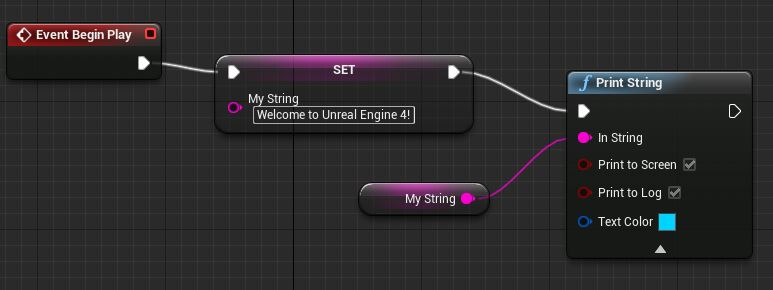
\includegraphics[width=1\textwidth]{figures/bp_example.jpg}
	\caption{Blueprint}
	\label{fig-bp-example}
\end{figure}

\end{description}

\section{Konwencja i architektura rozgrywki}
\label{sec:konwencja}
%\url{https://docs.unrealengine.com/latest/INT/Gameplay/Framework/index.html}
%\newline\url{https://docs.unrealengine.com/latest/INT/Gameplay/Framework/QuickReference/index.html}
%\newline obowiazkowo obrazek z dolu strony :D
Styl rozgrywki zależy od gry i wizji jej autora, jednak istnieją pewne cechy wspólne widoczne w niemal każdym tytule. Jest to na przykład sterowanie za pomocą urządzeń wejścia czy pewien zbiór zasad gry. Z tego powodu w UE4 przyjęto zaprezentowaną poniżej konwencję dotyczącą rozgrywki (rys. \ref{fig-gameplay-chart})\cite{docs-gameplay-framework}.
\begin{description}[itemsep=1\itemsep,parsep=1\parsep,partopsep=1\partopsep,topsep=1\topsep]
\item[Level:] W terminologii UE4 {\em level} jest zbiorem wszystkich obiektów, które gracz widzi lub może wejść z nimi w interakcje. Stanowi on reprezentację obszaru, w którym toczy się gra.
\item[Actor:]Jest to bazowa klasa dla każego obiektu, który można umieścić w {\em levelu}. Obiekty te nie muszą mieć fizycznej reprezentacji. Często zawierają dodatkowe komponenty ~({\em ActorComponents}) określające na przykład sposób porusza się obiektu. Oprócz tego {\em actor} posiada obsługę replikacji właściwości i wywołań funkcji przez sieć.
\item[Pawn:]Jest to {\em actor}, który może być kontrolowany przez gracza lub komputer. Stanowi ich fizyczną reprezentację w grach, które tego wymagają.
\item[Character:]Jest to humanoidalny {\em pawn} rozszerzony o następujące komponenty:
	\begin{description}
	\item[SkeletalMeshComponent] definiujący geometrię postaci w przypadku animacji szkieletowych,
	\item[CapsuleComponent] wykorzystywany przy kolizjach z innymi obiektami,
	\item[CharacterMovementComponent] opisujący ludzkie ruchy takie jak chodzenie, bieganie czy pływanie oraz właściwości związane z ruchem na przykład prędkość chodzenia czy wpływ grawitacji.
	\end{description}
\item[Controller:] jest to {\em aktor}, który po przejęciu {\em pawna} sprawuje nad nim kontrolę. Wyróżniamy dwa rodzaje: {\em PlayerController}, który stanowi interfejs między grającym, a sterowaną przez niego postacią (reprezentuje wolę gracza) oraz {\em AIController}, który decyduje o zachowaniach postaci na podstawie zaprogramowanych wcześniej drzew behawioralnych.
\newline {\em PlayerController} danego gracza w przypadku rozgrywki sieciowej występuje w dwóch instancjach: po jednej na serwerze oraz urządzeniu grającego, co należy brać pod uwagę podczas programowania tego elementu.
\item[HUD ({\em ang. head-up display}):] podręczne informacje wyświetlane na ekranie gracza na przykład jego obecny wynik, stany zdrowia widocznych postaci czy tak zwana minimapa.
\item[Camera:] decyduje o perspektywie, z której grający obserwuje {\em level}.
\item[GameMode:] zawiera informacje takie jak zasady gry czy warunki zwycięstwa. Nie powinien zawierać żadnych informacji potrzebnych klientom, ponieważ istnieje jedynie na serwerze. Decyduje również o tym, który {\em GameState} i {\em PlayerState} zostanie wykorzystany. Wybór {\em GameMode-a} zależy od wczytywanego {\em levelu}.
\item[GameState:] zawiera informacje o obecnym stanie rozgrywki na przykład czy mecz już się rozpoczął, wykonane misje, wyniki, listę graczy. {\em GameState} istnieje zarówno na serwerze jak i u klientów oraz jest replikowalny.
\item[PlayerState:] zawiera informacje o uczestniku rozgrywki na przykład jego imię, wynik czy zespół, do którego należy. Zarówno serwer jak i wszyscy klienci posiadają kopie {\em PlayerState-ów} dotyczących każdego grającego (co nie ma miejsca w przypadku {\em PlayerControllerów} -- każdy klient wie jedynie o swoim {\em PlayerControllerze}).
\item[GameInstance:] zawiera informacje o danej instancji gry. Istnieje jeden obiekt tej klasy na każdą uruchomioną grę i pozostaje on do dyspozycji aż do jej wyłączenia. Wczytywanie {\em leveli} nie ma wpływu na {\em GameInstance}, dzięki czemu klasa ta umożliwia przenoszenie informacji między {\em levelami}.
\end{description}
%dopisac cos ze trzymalismy sie tej konwencji i dalej prezentujemy jej wykorzystanie
Stosowanie się do tej konwencji zaprezentowano w rozdziale \ref{implementacja} skupiającym się na implementacji gry ,,thesis\_1``.

\section{Porównanie z innymi silnikami}
Bezpośrednim konkurentem dla UE4 jest silnik {\em Unity}. Jego główne różnice w stosunku do UE4 to:
\begin{itemize}
\item Pełniejsza i precyzyjniejsza dokumentacja.
\item Większa społeczność.
\item Lepsze narzędzia do produkcji gier 2D.
\item Bogatszy {\em AssetStore} czyli serwis, w którym użytkownicy mogą sprzedawać swoje assety (na przykład modele, dźwięki, animacje, gotowe systemy).
\item Język programowania {\em C\#}, co jest jednym z powodów niższej wydajności gier utworzonych w {\em Unity}.
\item Brak otwartego źródła.
\item Brak wielu funkcji w domyślnej konfiguracji silnika. Funkcje takie jak {\em visual scripting} czy drzewa behawioralne są stworzone przez społeczność, a za dostęp do nich trzeba zapłacić.
\item Rzadziej używany w wysokobudżetowych projektach.
\end{itemize}
Inną możliwością jest opracowanie własnego silnika od podstaw. W takim przypadku należy zadbać o podstawowe funkcje wymienione w podrozdziale \ref{czym-jest-silnik}. Wówczas przydatne są biblioteki {\em C++}: {\em SFML} oraz {\em SDL}. Osiągnięcie efektu porównywalnego do UE4 nawet dla dużego zespołu doświadczonych programistów będzie zadaniem czasochłonnym i kosztownym. Na to rozwiązanie decydują się głównie duże studia deweloperskie, które planują wykorzystać silnik do wielu projektów, a popularne silniki nie spełniają ich wymagań.

\begin{figure}
	\centering
		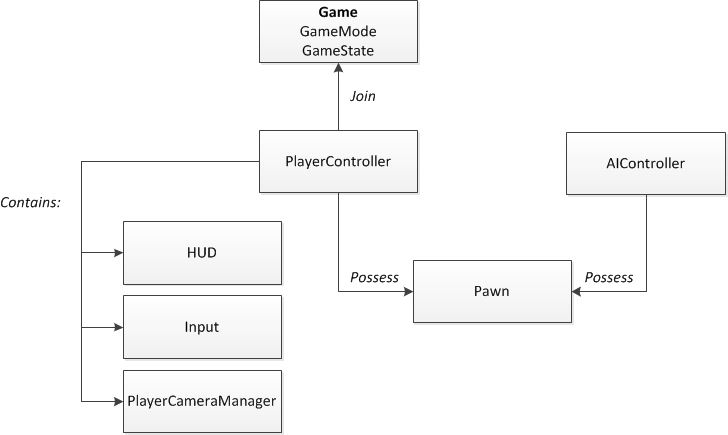
\includegraphics[width=1\textwidth]{figures/gameplay_chart.jpg}
	\caption{Diagram architektury rozgrywki}
	\label{fig-gameplay-chart}
\end{figure}

\chapter{Przykładowy przebieg rozgrywki w ,,thesis\_1``} %zeby opisac JAK zaimplementowalismy, trzeba najpierw opisac CO zaimplementowalismy

\begin{enumerate}
	\item Gracz pierwszy uruchamia grę po raz pierwszy, wobec czego jest przenoszony do menu opcji w celu wybrania ustawień (rys. \ref{settingsmenu}). Wpisuje swoje imię w odpowiednim polu, wybiera klasę postaci, zdolności, obrazek oraz czy będzie korzystał z klawiatury i myszki czy z kontrolera do gier (pada). Klika przycisk {\em Accept}, w katalogu gry powstaje plik z zapisem ustawień, gracz przenoszony jest do menu głównego.
	\item Gracz drugi uruchamiał już grę wcześniej, wobec czego posiada plik z zapisem. Po uruchomieniu przenoszony jest do menu głównego.
\item Gracz pierwszy w menu głównym klika przycisk {\em Host game}, a następnie ustala nazwę serwera, maksymalną liczbę graczy i metodę połączenia (Internet lub LAN). Aplikacja tego gracza będzie jednocześnie serwerem i klientem. Gracz zatwierdza przyciskiem {\em Accept}, po czym wczytuje mu się poziom, otrzymuje kontrolę nad swoją postacią, a serwer jest gotowy do przyjmowania klientów.
	\item Aplikacja Gracza drugi będzie klientem. W menu głównym gracz klika przycisk {\em Find game}, a następnie podaje adres IP Gracza pierwszego i zatwierdza przyciskiem {\em Connect}. Po chwili łączy się z serwerem i otrzymuje kontrolę nad swoją postacią.
	\item Obaj gracze prowadzą rozgrywkę(rys. \ref{gameplay1}), mogą chodzić, skakać, unikać oraz używać wybranych wcześniej zdolności. Sterowanie zależy od ustawień (mysz i klawiatura lub pad). Atakowanie postaci przeciwnika odbiera jej punkty zdrowia. Po utraceniu wszystkich punktów zdrowia dany gracz zostaje wyłączony z rozgrywki na siedem sekund, a wynik jego rywala jest zwiększany o jeden punkt. Obaj gracze widzą na swoich ekranach tablicę wyników aktualizowaną na bieżąco. Po upływie 7 sekund czasu gracz z powrotem otrzymuje kontrolę nad swoją postacią i gra jest kontynuowana.
	\item Gracze kończą rozgrywkę przyciskiem {\em X} w prawym górnym rogu okna. Gracz o najwyższym wyniku zostaje zwycięzcą.
\end{enumerate}
\begin{figure}
	\centering
		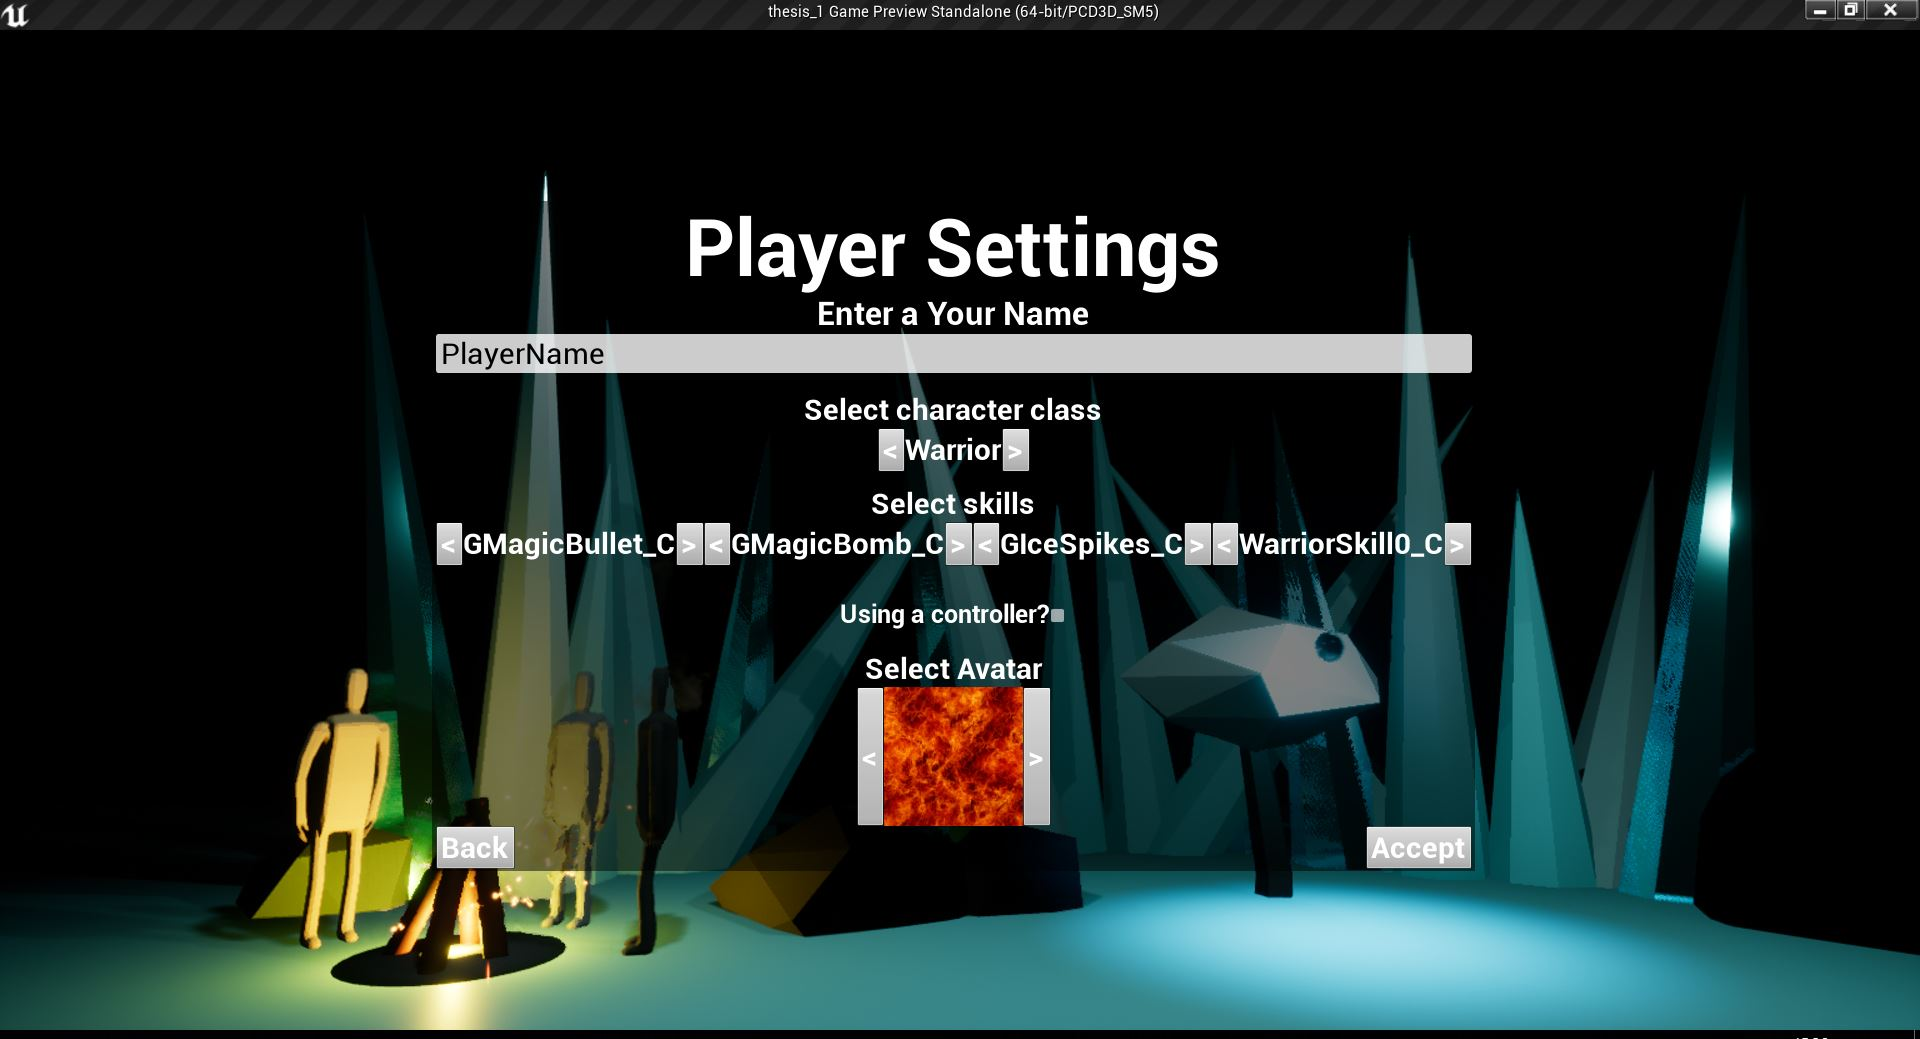
\includegraphics[width=1\textwidth]{figures/settingsmenu.jpg}
	\caption{Menu opcji}
	\label{settingsmenu}
\end{figure}
\begin{figure}
	\centering
		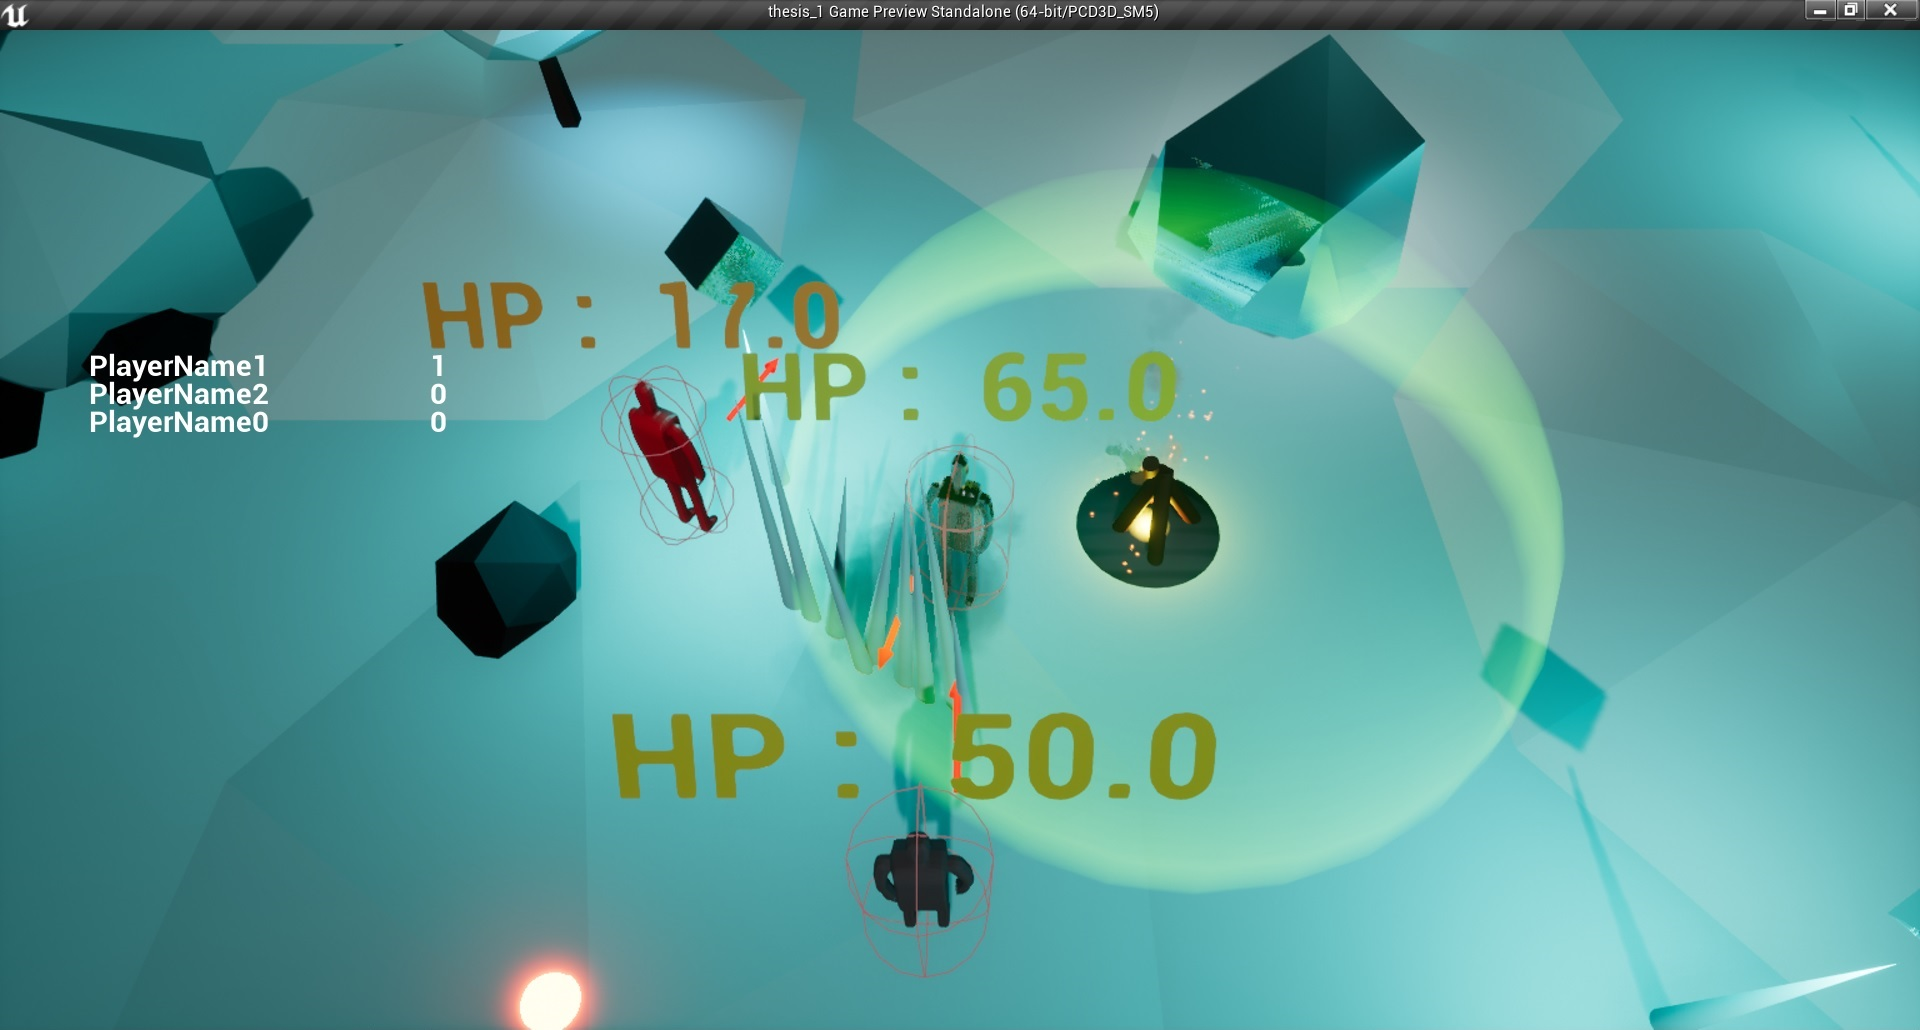
\includegraphics[width=1\textwidth]{figures/gameplay1.jpg}
	\caption{Rozgrywka}
	\label{gameplay1}
\end{figure}
\chapter{Opis implementacji gry ,,thesis\_1``}
\label{implementacja}
Opis dotyczy projektu dostępnego w publicznym repozytorium pod adresem \newline https://github.com/mszadko/thesis\_1.

\section{Uruchomienie gry i podstawowe funkcje}
Wywołanie pliku wykonywalnego z grą ({\em thesis\_1.exe}) powoduje uruchomienie silnika, utworzenie obiektu klasy {\em GameInfoInstance} (opisanej w podrozdziale \ref{gameinfoinstance}), a następnie wczytanie początkowego poziomu {\em MainMenu}, który wywołuje funkcję {\em SaveGameCheck} z {\em GameInfoInstance} sprawdzającą czy istnieje plik z zapisem gry (system opisany w podrozdziale \ref{sejwy}) i wyświetlający interfejs użytkownika. Na tym etapie grający otrzymuję kontrolę nad dalszym przebiegiem programu. Sprowadza się ona do wywołań funkcji z {\em GameInfoInstance} poprzez interfejs.
	\subsection{GameInfoInstance}
		\label{gameinfoinstance}
		Klasa {\em GameInfoInstance} dziedziczy po klasie {\em GameInstance} (opisanej w podrozdziale \ref{sec:konwencja}), zawiera podstawowe informacje wykorzystywane w innych obszarach gry (na przykład dostępne zdolności i klasy postaci wykorzystywane w systemie opisanym w podrozdziale \ref{wybor-postaci}) oraz odpowiada za wyświetlanie {\em widgetów} interfejsu (podrozdział \ref{interface}) i tworzenie oraz dołączanie do istniejących rozgrywek sieciowych (podrozdział \ref{networking}). Klasa została zaimplementowana za pomocą blueprintów.
	

\section{Interfejs}
	\label{interface}
	Podstawę interfejsu w UE4 stanowią {\em widgety} czyli elementy posiadające pewną logikę, które można wyświetlać w oknie użytkownika w warstwie interfejsu. Są to na przykład przyciski, listy, suwaki, pola tekstowe i tym podobne. Za pomocą edytora {\em widgetów} z podstawowych {\em widgetów} buduje się bardziej skomplikowane (na przykład menu główne lub tablica wyników), z których konstruuje się docelowy interfejs.
\newline \indent W przypadku gry ,,thesis\_1`` {\em widgety} wyświetlane są poprzez wywoływanie odpowiednich funkcji z {\em GameInfoInstance} (rys. \ref{fig-save-game-check}, \ref{fig-show-host-menu}). 
\newline \indent Z menu głównego grający ma możliwość przejścia do menu tworzenia lub dołączania do gry (rozdział \ref{networking}), menu opcji (rozdział \ref{wybor-postaci}) oraz zamknięcia gry. Wszystkie {\em widgety} zaimplementowane zostały za pomocą blueprintów.

	\begin{figure}
		\centering
			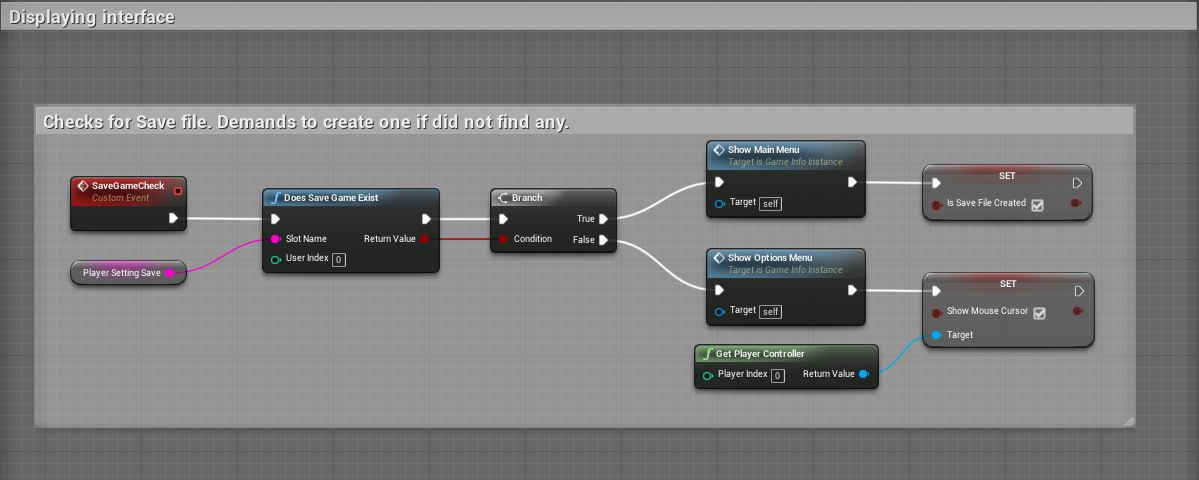
\includegraphics[width=1\textwidth]{figures/savegamecheck.jpg}
		\caption{Funkcja wywołująca wyświetlenie {\em widgetu} interfejsu wybranego na podstawie istnienia pliku zapisu stanu}
		\label{fig-save-game-check}
	\end{figure}
	
	\begin{figure}
		\centering
			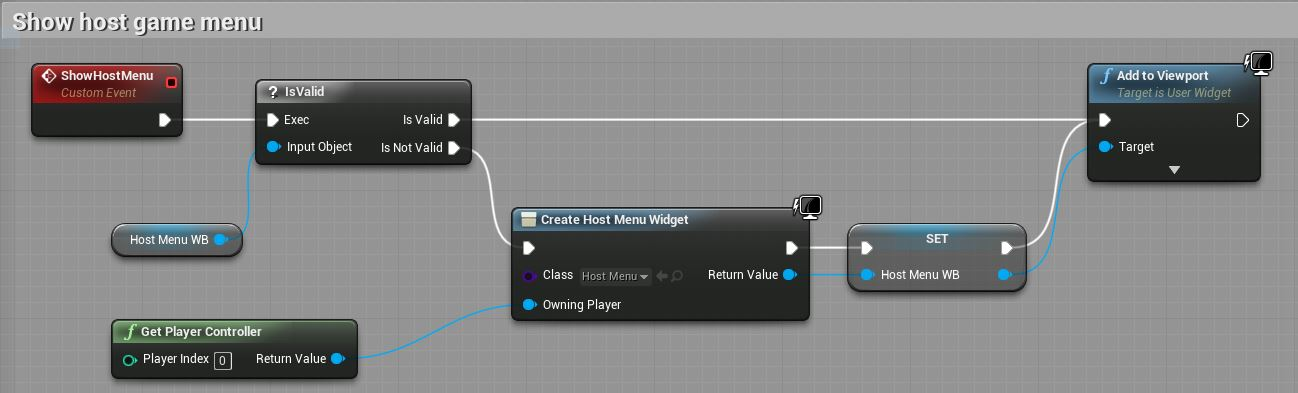
\includegraphics[width=1\textwidth]{figures/showhostmenu.jpg}
		\caption{Funkcja wyświetlająca {\em widget} interfejsu hostowania gry}
		\label{fig-show-host-menu}
	\end{figure}

\clearpage
\section{System zapisu stanu gry}
	\label{sejwy}
	W grze ,,thesis\_1`` zaimplementowano system zapisu gry, który umożliwia grającemu zachowanie swoich ustawień do kolejnego uruchomienia lub przeniesienia ich na inny komputer. System ten korzysta z klasy {\em PlayerSaveGame}, funkcji {\em SaveGameToSlot} i {\em LoadGameFromSlot} oraz struktury {\em PlayerInfo}. Obiekty klasy {\em PlayerSaveGame} są serializowane i deserializowane z pliku "thesis\_1/Saved/SaveGames/PlayerSettingsSave.sav" oraz posiadają w sobie strukturę {\em PlayerInfo}, w której przechowywane są ustawienia grającego: imię, obrazek, klasa postaci, rodzaj sterowania oraz zdolności.
	\newline Po uruchomieniu gry wywoływana jest funkcja {\em SaveGameCheck} z klasy {\em GameInfoInstance}, która jest odpowiedzialna za sprawdzenie, czy istnieje plik \newline "thesis\_1/Saved/SaveGames/PlayerSettingsSave.sav". Jeżeli nie istnieje, grający przenoszony jest do menu opcji, w którym wybiera ustawienia i powoduje stworzenie pliku z zapisem. Jeżeli plik ten istnieje, grający przenoszony jest do menu głównego, a dane z pliku wczytywane są przy wejściu do menu opcji (w celu wyświetlenia zapisanych ustawień) lub dołączeniu do rozgrywki (w celu utworzenia postaci oraz zdolności wybranych przez grającego). 
\section{Postacie i zdolności}
	\label{characters-skills}
Gra składa się wielu nieodzownych elementów, jednym z istotniejszych jest niewątpliwie postać którą gracz kontroluje.
	\subsection{Pawn, a PlayerController}
	Podczas tworzenia postaci pojawia się wiele pytań i problemów do rozwiązania.
Jednym z nich jest sposób zbierania danych od gracza. UE4 pozwala na obsługę danych wejściowych w klasach {\em Pawn} lub w {\em PlayerController}. Rzeczą wartą rozważenia jest sposób w jaki rozdzielimy obsługę wejścia pomiędzy tymi klasami\cite{docs-playercontroller}. W prostych przypadkach możliwa jest obsługa zebranych informacji o woli gracza całkowicie w klasie  {\em Pawn}. Jednak gdy sterowanie staje się skomplikowane, jego obsługa w {\em PlayerControllerze} jest nieunikniona.  {\em PlayerController} pozwala na przykład na sterowanie wieloma  {\em pawnami} na jednej maszynie czy dynamiczne przełączanie się pomiędzy postaciami.  Kolejną zaletą  {\em PlayerControllera} jest to, że jedna jego instancja jest przypisana do gracza przez całą rozgrywkę, a kontrolowane przez niego obiekty klasy  {\em Pawn} mogą się zmieniać. Na przykład podczas odradzania naszej postaci utworzony zostaje nowy obiekt klasy  {\em Pawn}, a kontroler pozostaje ten sam, więc dane, których nie chcemy stracić, takie jak zdobyte punkty czy złoto powinny być składową  {\em PlayerControllera}.
\newline \indent W grze ,,thesis\_1`` jako klasy bazowej do reprezentacji gracza użyto klasy  {\em Character}, a dane wejściowe są całkowicie obsługiwane przez  {\em PlayerController}.
	\subsection{Nazewnictwo klas C++}
	Utworzone klasy pochodne mają nazwy poprzedzone przedrostkiem {\em Base}. Konwencja ta odzwierciedla fakt, iż klasy {\em C++} zaimplementowane przez programistę są następnie wykorzystywane jako klasy bazowe blueprintów postaci. Wszystkie podstawowe umiejętności jak poruszanie się, skakanie czy obracanie się postaci zostały zaimplementowane za pomocą języka  {\em C++}, a następnie odziedziczone w blueprintach. Zyskano dzięki temu warstwę abstrakcji oddzielającą niezbędne linie kodu od dodatkowych zdolności postaci oraz łatwość zmian indywidualnych cech postaci za pomocą edytora blueprintów.
	\subsection{BaseCharacter}
	W celu rozwinięcia podstawowych możliwości klasy  {\em Character} udostępnionej przez silnik utworzono pochodną klasę  {\em BaseCharacter}. Głównym celem było pozwolenie graczom na dowolne dostosowanie zdolności postaci. Problem ten został rozwiązany za pomocą tablicy obiektów  {\em Skill}, które mają metody  {\em OnPress} oraz  {\em OnRelease}, wykonywane, gdy gracz -- odpowiednio -- naciska lub zwalnia odpowiedni przycisk.		
Dodane zostały również zmienne, które są używne przez silnik do odgrywania odpowiednich animacji takich jak animacja uniku czy animacja rzucania czaru oraz funkcje, które zmieniają wartości tych zmiennych na serwerze, gdy gracz na maszynie klienckiej wciśnie odpowiednie przyciski.
	\subsection{BasePlayerController i sterowanie}
	Klasa  {\em BasePlayerController} jest opracowanym na potrzeby projektu rozszerzeniem klasy  {\em PlayerController}. Jest ona odpowiedzialna między innymi za obsługę danych wejściowych, zebranych od gracza. 
Gracz ma do wyboru dwa sposoby kontrolowania swojej postaci. W zależności od ustawień w odpowiednim oknie interfejsu użytkownika gracz może korzystać z klawiatury oraz myszy lub z kontrolera gier. Sterowanie odbywa się za pomocą:
\begin{description}
\item[Klawiatury i myszy]
Postać można poruszać za pomocą klawiszy W, A, S oraz D i obrócona jest zawsze w kierunku kursora myszy. Klawisz F odpowiada za unik, a {\em spacja} za skok. Zdolności uruchamiane są przyciskami 1, 2, 3 i 4.
\item[Kontrolera Xbox One]
Drążki kontrolera odpowiadają za ruch i kierunek postaci. Przycisk A odpowiada za unik, a B za skok. Zdolności uruchamiane są przyciskami LT, LB, RT i RB.
\end{description}
Uruchamianie zdolności działa dwuetapowo. Podczas wciśnięcia klawisza odgrywana jest animacja oraz wykonywany jest kod metody {\em OnPress} z klasy {\em Skill}, który może wykonać całą logikę zdolności lub przygotować naszą postać do momentu gdy gracz zwolni przycisk. Następnie wykona się metoda {\em OnRelease}, która może pozostać pusta, dokończyć wykonanie zdolności lub przywrócić gracza do stanu sprzed kliknięcia przycisku.
\subsection{BaseCharacterMovementComponent}
{\em CharacterMovementComponent} jest komponentem klasy {\em Character}, odpowiedzialnym za przemieszczanie się postaci, który automatycznie obsługuje komunikację sieciową. Komponent ten umożliwia między innymi predykcję, replikację i korekcję ruchu. Działa on w następujący sposób \cite{docs-charactermovementcomponent}. Co klatkę wywoływana jest metoda {\em TickComponent}, gdzie obliczane są zmiany przyspieszenia oraz rotacji postaci. Następnie, w zależności od tego, czy program wykonywany jest na kliencie czy na serwerze, wywoływana jest metoda {\em PerformMovement} lub {\em ReplicateMoveToServer}. {\em ReplicateMoveToServer} dodaje ruch do listy oczekujących ruchów, następnie wywołuje metodę {\em PerformMovement} i replikuje ruch na serwer za pomocą zdalnie wywoływanej metody {\em ServerMove}. {\em ServerMove} przesuwa postać na serwerze w odpowiednie miejsce, a następnie oblicza dystans pomiędzy pozycją postaci na serwerze i na maszynie klienckiej. Jeżeli dystans jest większy niż dopuszczalny, serwer zdalnie wywołuje na kliencie metodę {\em ClientAdjustPosition}, która przesuwa postać w odpowiednie miejsce. Jeżeli dane korekcyjne dotrą do klienta, a jego pozycja zostanie poprawiona, metoda {\em ClientAdjustPosition} wykona ponownie wszystkie ruchy, które zostały dodane na listę ruchów oczekujących po ruchu, który został poprawiony przez serwer.
\newline \indent Dane o aktorze, takie, jak jego pozycja, prędkość czy rotacja, są replikowane na inne maszyny za pomocą standardowego mechanizmu replikacji. Oznacza to, że maszyny nie dostają potrzebnych im informacji co klatkę, co twórcy silnika rozwiązali za pomocą systemów predykcji i wygładzania. Systemy te wypełniają luki w danych spowodowane rozbieżnością między częstotliwościami renderowania klatek i replikowania danych. Predykcja polega na przesuwaniu obiektu klasy {\em Character} zgodnie z ostatnio otrzymanymi danymi na temat ruchu postaci. Gdy predykcja odbiega od rzeczywistych zmian, które zaszły na innych maszynach, UE4 nakłada na pozycję stopniowe korekty w celu uniknięcia nagłej jej zmiany.
\newline \indent Z powodu tych systemów wszystkie zdolności postaci, modyfikujące jej położenie, powinny zostać zaimplementowane poprzez rozszerzenie klasy {\em CharacterMovementComponent}.
W celu dodania możliwości uniku, polegającego na gwałtownym odskoku postaci w danym kierunku, opracowano klasę {\em BaseCharacterMovementComponent}. Implementacja polegała na nadpisaniu metod klasy bazowej \cite{uewiki-charmovement}. TickComponent oprócz swojego pierwotnego zadania sprawdza czy gracz wciska przycisk odpowiedzialny za unik. W takim przypadku dodawane są symulowane dane wejściowe, które naśladują poruszanie się gracza w odpowiednim kierunku. W celu zapewnienia szybszego poruszania się postaci podczas uniku, nadpisano metody {\em GetMaxSpeed} oraz {\em GetMaxAcceleration} tak, aby w zależności od zmiennej wskazującej na to czy postać wykonuje unik, zwracały różne wartości. Ponadto potrzebne było rozszerzenie klas używanych do predykcji i zapisywania ruchu na listę oczekujących w taki sposób, by ewentualna poprawa ruchu spowodowana opóźnieniami transmisji danych uwzględniła kliknięcie przez gracza przycisku uniku.
\clearpage
	\subsection{Skill}
	Jedną z głównych cech gry ,,thesis\_1`` jest możliwość wyboru czterech z wielu dostępnych zdolności do używania w trakcie rozgrywki. W tym celu powstała klasa {\em Skill} reprezentująca zdolność. Klasa ta powstała za pomocą kodu {\em C++} z myślą o rozszerzaniu jej blueprintami, co umożliwiają znaczniki {\em Blueprintable} oraz {\em BlueprintNativeEvent} użyte w nagłówku klasy. Każda klasa dziedzicząca po {\em Skill} reprezentuje jedną zdolność i nadpisuje bazowe funkcje {\em OnPress} oraz {\em OnRelease} logiką danej zdolności. Decyduje też o tym, które klasy postaci mogą używać danej zdolności.
	\subsection{Wybór postaci i zdolności}
		\label{wybor-postaci}
	Grający ma możliwość wyboru postaci oraz zdolności w menu opcji, które pobiera informacje o klasach postaci i zdolnościach z {\em GameInfoInstance}. Aby zapobiec sytuacji, w której wybrana została zdolność przeznaczona dla innej postaci niż obecnie wybrana, interfejs aktualizuje listę dostępnych zdolności przy każdej zmianie klasy postaci. Po zaakceptowaniu zmian tablica zdolności trafia do {\em PlayerInfo} oraz pliku z zapisem gry. Przy dołączeniu do rozgrywki informacje te trafiają do {\em PlayerControllera} za pomocą funkcji {\em LoadPlayerInfo}, a stamtąd do {\em Charactera} poprzez funkcję {\em ABaseCharacter::LoadSkills()} przy każdym jego odrodzeniu.

\section{Networking -- tworzenie oraz dołączanie do rozgrywki sieciowej}
	\label{networking}
,,thesis\_1`` jest grą sieciową i do kompletnej rozgrywki wymaga przynajmniej dwóch komputerów, z których jeden pełni rolę serwera, a pozostałe są klientami. W UE4 serwer może działać w jednym z dwóch trybów sieci \cite{docs-network-modes}:
\begin{description}
\item[NM\_DedicatedServer:]wymaga stworzenia oddzielnego oprogramowania serwera, które pozbawione jest między innymi elementów związanych z grafiką, dźwiękami czy wejściem. Dzięki temu więcej zasobów komputera wykorzystywanych jest na obliczenia związane z obsługą podłączonych klientów. Gracze do podłączenia i prowadzenia rozgrywki korzystają z oprogramowania klienckiego. Nie jest możliwe granie z poziomu serwera. To podejście stosowane jest w przypadku gier ze skomplikowaną, wymagającą komunikacją sieciową.

\item[NM\_ListenServer:]zarówno serwer i klienci korzystają z dokładnie tego samego oprogramowania, a komputer będący serwerem jest jednocześnie klientem. Wydajność jest niższa niż w przypadku serwera dedykowanego w zamian za możliwość prowadzenia rozgrywki z poziomu serwera.
\end{description}

W ,,thesis\_1`` wykorzystano tryb {\em NM\_ListenServer} ze względu na zapewnianą przez niego łatwość rozpoczęcia rozgrywki i niskie wymagania sieciowe gry. W implementacji sieciowych aspektów rozgrywki wykorzystywano głównie zdalne wywoływanie procedur, co wymaga sprecyzowania, czy mają one być wykonywane na serwerze czy na kliencie, sprawdzania roli instancji gry to znaczy czy obecnie wykonujemy kod na serwerze czy na~kliencie~(rys. \ref{switch-has-authority}) oraz oznaczania {\em actorów} do replikacji czyli przesyłania informacji o nich między serwerem, a klientami.
\newline \indent Utworzenie serwera odbywa się poprzez menu {\em Host game}, a jego widoczność zależy od konfiguracji sieciowej gracza i jego dostawcy Internetu. Gra ,,thesis\_1`` korzysta z portu 7777 (domyślnego w UE4).
\newline \indent Łączenie z serwerem inicjowane jest w menu {\em Find game} poprzez automatyczne wyszukanie gry w sieci lokalnej lub podanie adresu IP serwera w Internecie lub sieci lokalnej. Następnie na serwerze wykonywana jest funkcja {\em OnPostLogin} (rys. \ref{switch-has-authority}), która inicjuje wczytanie danych z pliku łączącego się gracza, pobiera je od niego i na ich podstawie przydziela mu postać.

\begin{figure}
		\centering
			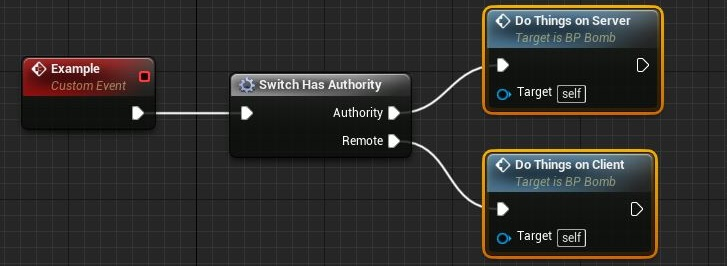
\includegraphics[width=0.7\textwidth]{figures/switchhasauth.jpg}
		\caption{Blueprint, w którym logika zależy od roli}
		\label{switch-has-authority}
\end{figure}

\section{Modele i Animacje }
Wartym zaznaczenia jest fakt, że głównym celem tworzenia modeli i animacji było zapoznanie się z narzędziami oraz samym procesem tworzenia tej części gier komputerowych. Podczas pracy nad projektem skupiono uwagę na aspektach technicznych. Znaczną część elementów {\em levelu} udało się stworzyć za pomocą obracania i skalowania gotowych kształtów udostępnionych w UE4. Bardziej skomplikowane kształty wymagały wymodelowania w osobnym oprogramowaniu dedykowanym do tego celu. Do stworzenia modeli i animacji użytych w projekcie wykorzystano oprogramowanie Blender w wersji 2.79.

	\subsection{Modelowanie}
Modelowanie w Blenderze polega na przemieszczaniu odpowiednich wierzchołków podstawowych kształtów, takich jak sfera czy sześcian, aż do momentu otrzymania docelowego obiektu. Animowanie tak wymodelowanej siatki obiektu (rys. \ref{blender-model}) jest praktycznie niemożliwe.
	\subsection{Rigging}
Następnym krokiem jest proces nazwany {\em rigging}\cite{whats-rigging}. {\em Rigging} polega na wyposażeniu modelu w kości, stawy oraz stworzeniu mapy wag informującej o tym jak dane kości mają wpływać na kształt modelu (rys. \ref{blender-rigging}). Umożliwia to animowanie obiektu.
\begin{figure}
		\centering
			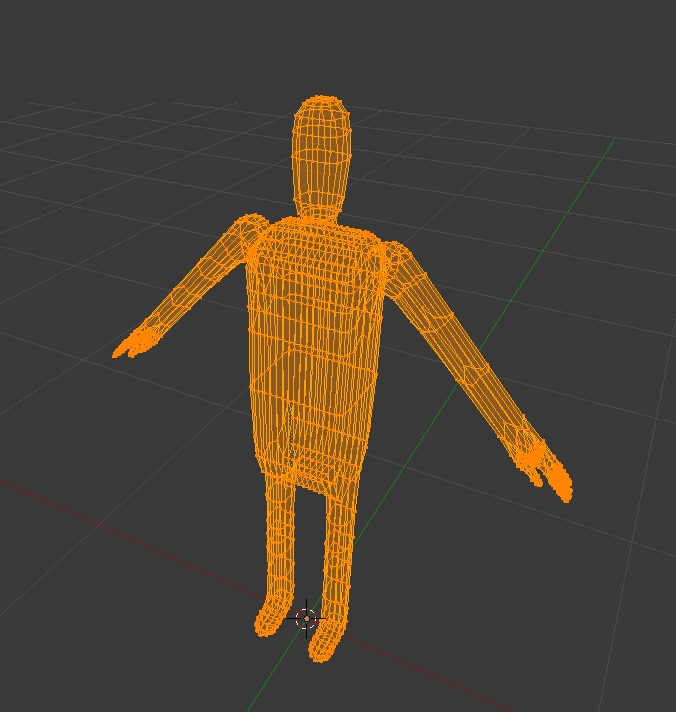
\includegraphics[width=0.44\textwidth]{figures/adimodel.jpg}
		\caption{Model postaci wykorzystany w grze}
		\label{blender-model}
\end{figure}
\begin{figure}
		\centering
			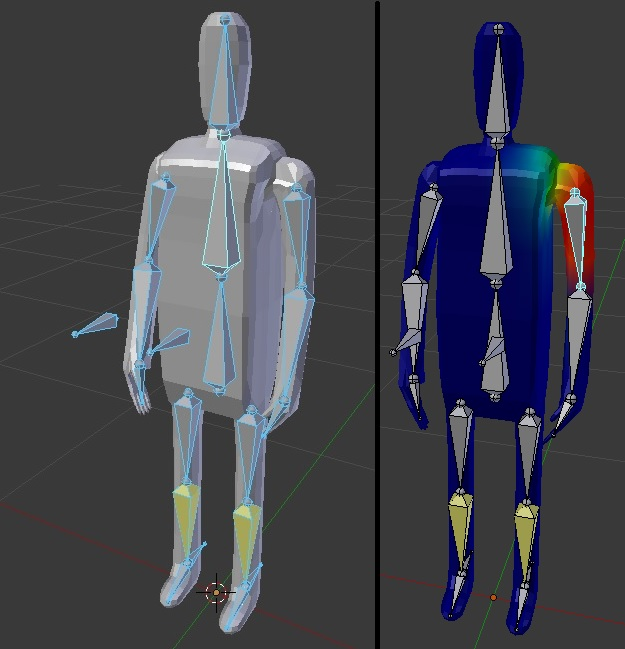
\includegraphics[width=0.44\textwidth]{figures/adirig.jpg}
		\caption{Kości oraz stawy użyte w modelu (po lewej) oraz mapa wag dla jednej z kości (po prawej)}
		\label{blender-rigging}
\end{figure}
\clearpage
	\subsection{Animacje}
\begin{figure}
		\centering
			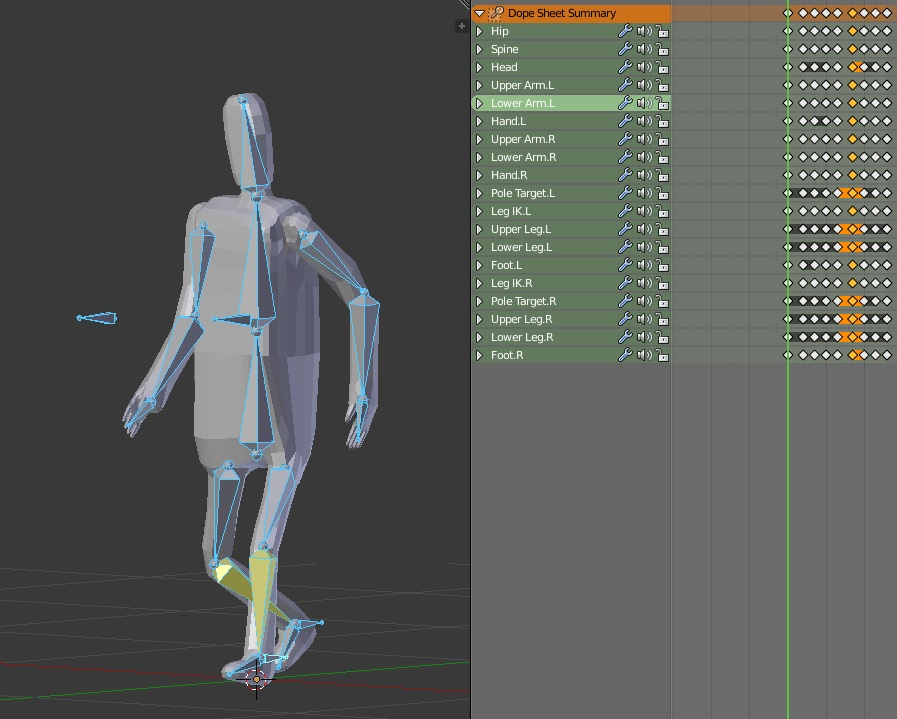
\includegraphics[width=1\textwidth]{figures/adiwalk.jpg}
		\caption{Jedna z klatek animacji chodzenia}
		\label{blender-anim}
\end{figure}
Proces tworzenia animacji polega na ustawianiu kości w odpowiednich pozach i zapisywaniu ich zmian w rotacji oraz położeniu (rys. \ref{blender-anim}). 
W animacjach nawet podstawowych ruchów pojawia się wiele problemów do rozwiązania. Przykładem może być animacja skoku, w której problematyczny jest zmienny czas przebywania postaci w powietrzu. Animacja zeskakiwania z wysokiej przeszkody powinna trwać dłużej niż animacja wskakiwania na przeszkodę. Problem ten został rozwiązany za pomocą rozbicia sekwencji skoku na 3 oddzielne animacje – wybicie się, przebywanie w powietrzu oraz lądowanie. Ostatnia klatka wybicia jest jednocześnie pierwszą i ostatnią klatką przebywania w powietrzu oraz pierwszą klatką lądowania. Pozwoliło to na zapętlone odgrywanie animacji przebywania w powietrzu z płynnymi przejściami pomiędzy wybiciem, a lądowaniem.

\section{Udźwiękowienie}
Odtwarzanie dźwięków w grze obsłużono dwoma funkcjami. W przypadku muzyki i dźwięku towarzyszącego zdobyciu punktu jest to funkcja {\em PlaySound2D}, która odtwarza dźwięk u tych klientów, u których została wywołana. Dźwięki związane ze zdolnościami i ogniskiem odtwarzane są za pomocą funkcji {\em SpawnSoundAtLocation}, dzięki czemu słyszą je jedynie gracze będący blisko źródła dźwięku.
\newline \indent Użyto następujących dźwięków pochodzących ze strony internetowej freesound.org:
\begin{itemize}
\item ,,06673 electronic flipper bonus.wav`` autorstwa Robinhood76 (licencja CC BY-NC)
\item ,,avl03.wav`` autorstwa blaukreuz (licencja CC 0)
\item ,,shatter a wine glass`` autorstwa edhutschek (licencja CC 0)
\item ,,jumping`` autorstwa fins (licencja CC 0)
\end{itemize}

\chapter{Dalszy rozwój gry}
W kolejnych podrozdziałach zaprezentowano możliwości dalszego rozwoju gry. Poprzez implementację nowych klas postaci, zdolności oraz postaci sterowanych przez komputer można urozmaicić rozgrywkę, a nawet całkowicie zmienić jej charakter z rywalizacji między graczami na współpracę.

\section{Klasy postaci i zdolności}
Klasy {\em Skill} oraz {\em BaseCharacter} zostały opracowane z myślą o ułatwieniu dalszego rozwoju gry. Utworzenie nowej postaci, różniącej się od dotychczasowych na przykład liczbą punktów zdrowia czy prędkością, sprowadza się do odziedziczenia klasy bazowej i zmiany wartości odpowiednich zmiennych. Utworzenie zdolności różniącej się na przykład liczbą zadawanych obrażen czy czasem, który należy odczekać przed ponownym użyciem zdolności, to również kwestia zmiany pojedyńczych zmiennych. W przypadku implementacji zdolności o zupełnie nowej logice za wzór służą zdolności dostępne w finalnej wersji gry.
\newline \indent Nowo opracowane postaci i zdolności muszą zostać umieszczone w -- odpowiednio -- słowniku {\em CharacterClasses} lub tablicy {\em Skills} w blueprincie {\em GameInfoInstance}, aby były widoczne w grze.

\section{Sztuczna inteligencja}
Możliwe jest również wykorzystanie dostępnego w UE4 mechanizmu drzew behawioralnych w celu zaimplementowania postaci sterowanych przez komputer. Sprowadza się to do utworzenia następujących elementów \cite{docs-behavior-tree-quick-start}:
\begin{itemize}
\item Nowa postać dziedzicząca po {\em BaseCharacter}
\item {\em NavMesh} określający, w które miejsca postać może się przemieścić
\item Drzewo behawioralne zwracające konkretne zachowanie na podstawie danych wejściowych
\item {\em Blackboard} będący zbiorem danych dla drzewa behawioralnego
\item {\em AIController} będący odpowiednikiem {\em PlayerControllera} i spinający wyżej wymienione elementy. {\em AIController} decyduje o wykorzystywanym {\em Blackboardzie} i drzewie behawioralnym oraz inicjuje dane zachowanie w postaci.
\end{itemize}

\chapter{Napotkane problemy}
Niejednokrotnie trudności sprawiała niedokładna dokumentacja silnika lub nawet jej brak. W takich sytuacjach pomocne okazywały się rady społeczności skupionej wokół UE4 oraz otwarte źródło silnika.
\newline \indent Problem stanowiło również korzystanie z systemu kontroli wersji Git, ponieważ nie jest on przystosowany do obsługi plików innych niż tekstowe. Skutkiem jest utrudnione rozwiązywanie ewentualnych konfliktów powstałych w plikach związanych na przykład z blueprintami czy modelami. Problem ten będzie dotkliwszy dla większych zespołów.

\chapter{Podsumowanie i wnioski}
Tworzenie gier nie należy do zadań łatwych oraz szybkich. Podczas pracy nad projektem pojawiło się wiele dodatkowych problemów, przez co lista założonych na początku opcji gry musiała zostać skrócona. Jednym z nich był wysoki próg wejścia UE4. Przed rozpoczęciem pracy nad docelowym projektem, stworzonych zostało kilka mniejszych gier wzorowanych na przykładowych projektach z dokumentacji\cite{docs-tutorials}, które miały na celu zaznajomienie autorów z konwencjami, możliwościami silnika oraz systemem sieciowym. Czas tworzenia wydłużało dodatkowo scalanie podsystemów utworzonych przez poszczególnych autorów gry. Gry wideo są skomplikowanymi programami komputerowymi z duża liczbą połączeń pomiędzy danymi elementami gry. System zapisu jest na przykład zależny od wybranych opcji w interfejsie użytkownika, który z koleji jest powiązany z klasą postaci. Ze względu na dużą liczbę powiązań pomiędzy różnymi elementami projektu, nawet najmniejsze zmiany mogły spowodować powstawanie różnorakich błędów, przez co dużą część czasu poświecono na proces testowania każdego nowo dodanego elementu.
\newline \indent Silnik UE4 umożliwił stworzenie prostej sieciowej gry w stosunkowo niedługim czasie. Gra była zaprojektowana z myślą o jej dalszym rozwoju co wraz ze znajomością silnika UE4 pozwala na  sprawne dodawanie kolejnych elementów rozgrywki. Osiągniety efekt nie byłby możliwy bez wykorzystania profesjonalnych narzędzi takich jak UE4 czy Blender.
 \chapter{Zawartość płyty}
Na płycię znajduję się gotowa do uruchomienia wersja gry oraz folder zawierający wszystkie pliki stworzone na potrzeby projektu. W folderze znależć można między innymi kod źródłowy oraz pliki blueprintów zawierające większość stworzonej logiki gry. Na przykład blueprinty interfejsu użytkownika, postaci, interaktywnych elementów środowiska czy dostępnych umiejętności. W plikach znajdują się również {\em level} na którym toczy się rozgrywka, modele, animacje oraz dźwięki wykorzystane w grze. 

\begin{thebibliography}{9}

\bibitem{learning-unreal}
Joanna Lee, \textit{Learning Unreal Engine Game Development}, Packt Publishing, 2016

\bibitem{perelki}
Mark DeLoura, \textit{Perełki Programowania Gier, Vademecum profesjonalisty, Tom I, strony 17-21.} Helion, 2002

\bibitem{szkolacpp}
Stephen Prata, \textit{Język C++, Szkoła programowania, wydanie VI, strony 21-37.} Helion, 2013

\bibitem{docs-ue4-features}
\textit{Engine Features}. \url{https://docs.unrealengine.com/latest/INT/Engine/index.html} (dostęp 30.12.2017)

\bibitem{docs-tutorials}
\textit{UE4 Documentation Tutorials}. \url{https://docs.unrealengine.com/latest/INT/Videos/} (dostęp 14.01.2018)

\bibitem{docs-blueprints}
\textit{UE4 Documentation Blueprints Visual Scripting}. \url{https://docs.unrealengine.com/latest/INT/Engine/Blueprints/index.html} (dostęp 30.12.2017)

\bibitem{docs-playercontroller}
\textit{UE4 Documentation Player Controller}. \url{https://docs.unrealengine.com/latest/INT/Gameplay/Framework/Controller/PlayerController/}  (dostęp 3.01.2018)

\bibitem{docs-charactermovementcomponent}
\textit{UE4 Documentation Character Movement Component}.  \url{https://docs.unrealengine.com/latest/INT/Gameplay/Networking/CharacterMovementComponent/index.html}  (dostęp 3.01.2018)

\bibitem{docs-network-modes}
\textit{UE4 Documentation Networking Overview}. \url{https://docs.unrealengine.com/latest/INT/Gameplay/Networking/Overview/} (dostęp 05.01.2018)

\bibitem{docs-profiler}
\textit{UE4 Documentation Performance and Profiling}. \url{https://docs.unrealengine.com/latest/INT/Engine/Performance/}  (dostęp 3.01.2018)

\bibitem{docs-gameplay-framework}
\textit{UE4 Documentation Gameplay Framework Quick Reference}. \url{https://docs.unrealengine.com/latest/INT/Gameplay/Framework/QuickReference/index.html} (dostęp 31.12.2017)

\bibitem{docs-behavior-tree-quick-start}
\textit{UE4 Documentation Behavior Tree Quick Start Guide}. \url{https://docs.unrealengine.com/latest/INT/Engine/AI/BehaviorTrees/QuickStart/index.html} (dostęp 14.01.2018)

\bibitem{wiki-game-engine}
\textit{,,Game engine``, Wikipedia}. \url{https://en.wikipedia.org/wiki/Game_engine} {\mbox(dostęp 29.12.2017)}

\bibitem{uewiki-charmovement}
\textit{UE4 Wiki - Authoritative Networked Character Movement}. \url{https://wiki.unrealengine.com/Authoritative_Networked_Character_Movement}  (dostęp 3.01.2018)

\bibitem{unreal-wiki-replication}
\textit{Everything you ever wanted to know about replication (but were afraid to ask)}. \url{https://wiki.beyondunreal.com/Everything_you_ever_wanted_to_know_about_replication_\%28but_were_afraid_to_ask\%29#Function_call_replication_-_Sending_messages_between_server_and_client} (dostęp 30.12.2017)

\bibitem{nasdaq-video-games-industry}
Trevir Nath, \textit{Investing in Video Games: This Industry Pulls In More Revenue Than Movies, Music}.
\url{http://www.nasdaq.com/article/investing-in-video-games-this-industry-pulls-in-more-revenue-than-movies-music-cm634585} {\mbox(dostęp 29.12.2017)}

\bibitem{the-human-race}
\textit{The Human Race – An Inside Look at the Technology Behind the Groundbreaking Real-Time Film from Epic Games, The Mill and Chevrolet}. \url{https://www.unrealengine.com/en-US/showcase/the-human-race-an-inside-look-at-the-technology-behind-the-groundbreaking-real-time-film-from-epic-games-the-mill-and-chevrolet} (dostęp 30.12.2017)

\bibitem{ikea-vr}
\textit{Virtual Reality- Into the magic}. \url{http://www.ikea.com/ms/en_US/this-is-ikea/ikea-highlights/Virtual-reality/index.html} (dostęp 30.12.2017)

\bibitem{whats-rigging}
Justin Slick, \textit{What is Rigging? Preparing a 3D Model For Animation }. \url{https://www.lifewire.com/what-is-rigging-2095}  (dostęp 3.01.2018)






\end{thebibliography}


\beforelastpage
 \thispagestyle{empty} \newpage \null \thispagestyle{empty}
\end{document} 
